\documentclass[a3paper,12pt]{article}

\usepackage{amsmath} %Для многострочных формул
\usepackage[utf8]{inputenc} %Включаем поддержку UTF8
\usepackage[english,russian]{babel} %Локализация
\usepackage{multicol} %Несколько колонок
\usepackage{graphicx} %Картинки
\usepackage{caption} %Подпись под рисунком
\usepackage[left=1cm,right=1cm,top=2cm,bottom=2cm,bindingoffset=0cm]{geometry} %Поля
\usepackage{lettrine} %Первая буква в абзаце

\graphicspath{{pictures/}} %Путь к графическим файлам
\DeclareGraphicsExtensions{.png} %Список расширений
\setlength{\parskip}{1pt} %Интервал между абзацами
\pagestyle{empty} % нумерация страниц выкл.

%Положение подписей
\usepackage{floatrow}
\floatsetup[table]{capposition=top,margins=raggedright}
\floatsetup[figure]{capposition=bottom,margins=raggedleft}

%Доп задание
\usepackage{tikz}
\usetikzlibrary{automata,positioning}

\begin{document}
	\begin{center}
	
\includegraphics[scale=0.5]{logo.png}
	\vspace{5 cm}
	
	\LARGE Лабораторная работа №7\\
	Работа с системой компьютерной вёрстки TEX
	\vfill
\end{center}
\begin{flushright}
	\large
	Выполнил: Канторов Всеволод Сергеевич\\
	Группа: P3112\\
	Преподователь: Малышева Т.А.\\
	\vfill
\end{flushright}

\begin{center}
	\large Санкт-Петербург, 2019
\end{center}

\newpage

	\begin{center}
	\LARGE ШКОЛА В <<КВАНТЕ>>
	\noindent{\rule{0.9\paperwidth}{0.4pt}}	
\end{center}

\begin{multicols}{3}
	
	\begin{minipage}[t]{8cm}
		\begin{center}
			\Huge Теорема Mенелая\\ для тетраэдра\\
			\large И.Габович
		\end{center}
		\vspace{5mm}
	\end{minipage}
	
	\lettrine{\textbf{В}}{} НEКОТОРЫХ  пособиях по геометрии приводится планиметрическая теорема, называемая теоремой Менелая\footnote{Менелай Александрийский (1 -- 2\\ в. н. э.)-- греческий математик и\\ астроном.}. Приведем ее формулировку.
	
	\textbf{Теорема 1.} Если P, Q и R -- соответственно точки пересечения каждой из сторон BC, CA и AB (или их продолжений) треугольника ABC с некоторой прямой, то
	$$\frac{BR}{RA} \cdot \frac{AQ}{QC} \cdot \frac{CP}{PB} = 1.$$
	
	Эта теорема редко используется в решении планиметрических задач (в частности, таких, которые обычно предлагаются на вступительных экзаменах в вузы) и поэтому она мало известна даже учащимся, проявляющим повышенный интерес к изучению математики. Предлагаем читателям самостоятельно доказать эту теорему.
	
	Еще менее известна стереометрическая теорема Менелая для произвольного тетраэдра, которая, как будет показано ниже, весьма эффективно используется при решении некоторых задач.
	
	Доказательству этой теоремы и ее применению в решении задач с посвящена данная статья. Начнем с формулировки.
	
	\textbf{Теорема 2.} В произвольном тетраэдре KLMN точки A, B, C и D принадлежат ребрам KN, NL, LM и MK соответственно (рис. \ref{1}). Для того
	\begin{figure}[H]
		\begin{minipage}{\linewidth}
			\centering
			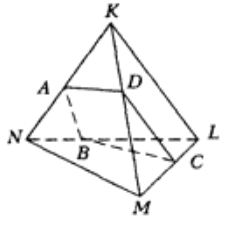
\includegraphics[width=0.6\linewidth]{1}
			\caption{}
			\label{1}
		\end{minipage}
	\end{figure}
	\begin{figure}[H]
		\begin{minipage}{\linewidth}
				\centering
				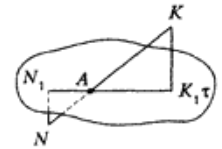
\includegraphics[width=0.6\linewidth]{2}
				\caption{}
				\label{2}
			\end{minipage}
	\end{figure}
	чтобы точки A, B, C и D принадлежали одной плоскости, необходимо и достаточно, чтобы выполнялось следующее равенство:
	\begin{equation}
			\frac{KA}{AN} \cdot \frac{NB}{BL} \cdot \frac{LC}{CM} \cdot \frac{MD}{DK} = 1.
			\label{eq1}
		\end{equation}
	
	\textbf{Доказательство.} \textit{Необходимость.} Пусть четырехугольник ABCD -- сечение данного тетраэдра некоторой плоскостью $\gamma$ (на рисунке не показанной). Проведем $KK_1, NN_1, MM_1 \text{ и } LL_1$ -- перпендикуляры к плоскости $\gamma$. Рассмотрим <<фрагмент>> -- пересечение ребра KN с плоскостью $\gamma$ (рис. \ref{2}). Очевидно, что $\bigtriangleup KK_1A \sim\bigtriangleup NN_1A$. Из подобия этих треугольников следует, что
	\[\frac{KA}{AN} = \frac{KK_1}{NN_1}.\]
	Аналогично доказывается, что
	\[\frac{NB}{BL} = \frac{NN_1}{LL_1},\hspace{5mm} \frac{LC}{CM} = \frac{LL_1}{MM_1},\] \[\frac{MD}{DK} = \frac{MM_1}{KK_1}.\]
	Перемножив по частям выписанные выше равенства, получим равенство(\ref{eq1}).
	
	\textit{Достаточность.} Предположим, что выполняется равенство (\ref{eq1}), но точки A, B, C и D не лежат в одной плоскости. Проведем через точки B, C и D плоскость (назовем ее $\sigma$), которая пересечет ребро KN в некоторой точке $A_1$, отличной от точки A (в силу сделанного выше предположения). Поэтому $KA_1 : A_1N \neq KA : AN$, вследствие чего равенство (\ref{eq1}) для точек $A_1$, B, C и D выполняться не будет. Поскольку мы пришли к противоречию с исходным условием (не выполняется равенство (\ref{eq1})), то наше предположение ложно и, следовательно, плоскость $\sigma$ пройдет через точку A.
		
	Покажем теперь применение теоремы 2 к решению стереометрических задач.
		
	\textbf{Задача 1.} Втетраэдре ZABC точки M, N и P принадлежат ребрам ZA, AB и BC соответственно (рис. \ref{3}) причем $ZM : MA = 5 : 4, AN : NB = 2 : 5 \text{ и } BP : PC = 1 : 2$. Через точки M, N и P проведена плоскость $\gamma$. В каком отвношении эта плоскость делит объем тeтраэдра?

	\textbf{Решение.} Пусть плоскость $\gamma$ (на рисунке не показанная) пересечет ребро ZC в точке Q. Четырехугольник MNPQ -- сечение данного тетраэдра плоскостью  $\gamma$. Определим, в каком отношении точка Q делит ребро ZC. На основании равенства (\ref{eq1}) и данных 
	\begin{figure}[H]
		\begin{minipage}{\linewidth}
				\centering
				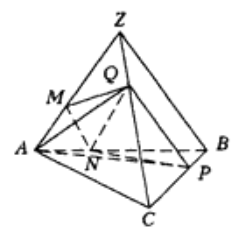
\includegraphics[width=0.6\linewidth]{3}
				\caption{}
				\label{3}
			\end{minipage}
	\end{figure}
	условия имеем
	\[\frac{ZM}{MA} \cdot \frac{AN}{NB} \cdot \frac{BP}{PC} \cdot \frac{CQ}{QZ} = 1,\]
	или 
	\[\frac{5}{4} \cdot \frac{2}{5} \cdot \frac{1}{2} \cdot \frac{CQ}{QZ} = 1,\]
	откуда
	\[CQ : QZ = 4 : 1.\]
	
	В многограннике MANPCQ проведем сечение через ребро AN и вершиной Q. Это сечение разбивает рассматриваемый многогранник на треугольную пирамиду QAMN и четырехугольную пирамиду QANPC, которая диагональнм сечением AQP разбивается на две трекгольные пирамиды: QAPC и QAPN.
		
	Пусть S -- площадь грани ABC, H -- длинна высоты тетраэдра, проведенной из вершины Z (сама высота на рисунке не показана), V -- объем данного тетраэдра.
	
	Определим объемы трех получанных выше треугольных пирамид. Для пирамиды QAPC
	\[V_{QAPC} = \frac{1}{3} S_{\bigtriangleup APC} \cdot H_Q,\]
	где $H_Q$ -- длина высоты треугольной пирамиды QAPC, проведенной из вершины Q на плоскость грани APC (на рисунке также не показанной). Лугко сообразить, что $H_Q = \frac{4}{5} H $. Тогда
	\begin{multline*}
			V_{QAPC} = \frac{1}{3} \left(\frac{2}{3} S\right) \cdot \frac{4}{5} H = \\ = \frac{8}{15} \left(\frac{1}{3} SH\right) = \frac{8}{15} V.
		\end{multline*}
	Аналогично,
	\begin{multline*}
			V_{QAPN} = \frac{1}{3} S_{\bigtriangleup APN} \cdot H_Q = \\ = \frac{1}{3} \left(\frac{2}{7} S_{\bigtriangleup ABP}\right) \cdot \frac{4}{5} H = \\ = \frac{8}{105} \cdot \left(\frac{1}{3}S\cdot H\right) = \frac{8}{105} V.
		\end{multline*}
	
	Пусть далее $S_1$ -- площадь грани ZAB, $H_1$ -- длина высоты данного тетраэдра, проведенной из вершины C на плоскость грани ZAB.
\end{multicols}

\newpage

\begin{table}
	\begin{tabular}{|l|c|c|c|c|c|c|c|}
		\hline
		& \multicolumn{7}{c|}{Задача} \\
		\hline
		\multicolumn{1}{|c|}{Участник} & 1 & 2 & 3 & 4 & 5 & 6 & $\sum$ \\
		\hline
		Николай Дуров & 7 & 7 & 7 & 7 & 2 & 7 & 37 \\
		\hline
		Вероника Есаулова & 4 & 7 & 3 & 7 & 1 & 3 & 25 \\
		\hline
		Юрий Макарычев & 6 & 7 & 5 & 1 & 0 & 0 & 19 \\
		\hline
		Сергей Норин & 7 & 7 & 7 & 7 & 1 & 7 & 36 \\
		\hline
		Елена Рудо & 2 & 1 & 6 & 7 & 0 & 7 & 23 \\
		\hline
		Константин Салихов & 2 & 7 & 5 & 7 & 1 & 0 & 22 \\
		\hline
	\end{tabular}
	\caption{}
\end{table}

\centering
\begin{tikzpicture}[node distance=4cm, auto]
	\node[state] (b1) {$b_1$};
	\node[state,right of=b1] (b2) {$b_2$};
	\node[state,right of=b2] (b3) {$b_3$};
	\node[state,below of=b1] (b4) {$b_4$};
	\node[state,right of=b4] (b5) {$b_5$};
	\node[state,right of=b5] (b6) {$b_6$};
	
	\path[->] (b1) edge[loop left] node {$z_1$} (b1);
	\path[->] (b2) edge[loop above] node {$z_2$} (b2);
	\path[->] (b4) edge[loop left] node {$z_3$} (b4);
	
	\path[->] (b1) edge node {$z_3$} (b2);
	\path[->] (b1) edge node {$z_2$} (b5);
	\path[->] (b4) edge node {$z_1$} (b1);
	\path[->] (b5) edge node {$z_2$} (b4);
	\path[->] (b5) edge node[near start] {$z_3$} (b3);
	\path[->] (b3) edge node {$z_2$} (b2);
	\path[->] (b2) edge node[near start] {$z_1$} (b6);
	\path[->] (b6) edge node {$z_3$} (b3);
	
	\path[->] (b6) edge[bend left] node {$z_2$} (b4);
	\path[->] (b3) edge[bend left] node {$z_1$} (b6);
\end{tikzpicture}

\sqrt[5]{\dfrac{x^2 + 1}{2}}

\end{document}